%!TeX root=../pridetop.tex
\chapter[Chapter \thechapter]{}
	
\begin{figure}[t!]
\centering
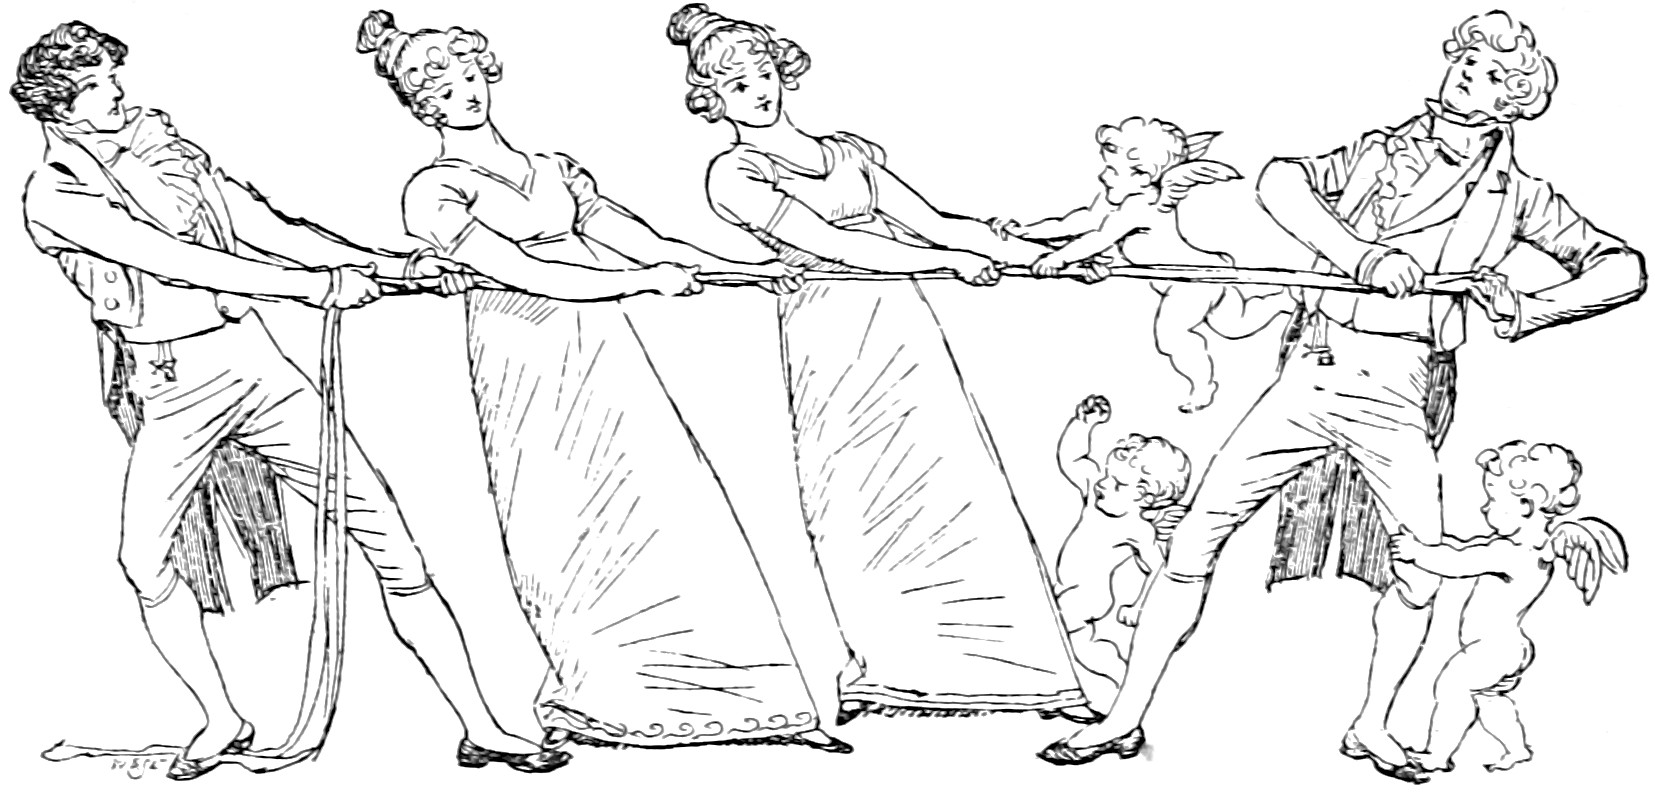
\includegraphics[width=\linewidth]{24top}
\captionlistentry{Headpiece to Chapter \thechapter}
\end{figure}


\lettrine[lines=6,image=true]{initials/chap24m}{iss}  Bingley's letter arrived, and put an end to doubt. The very first sentence conveyed the assurance of their being all settled in London for the winter, and concluded with her brother's regret at not having had time to pay his respects to his friends in Hertfordshire before he left the country.

\zz
Hope was over, entirely over; and when Jane could attend to the rest of the letter, she found little, except the professed affection of the writer, that could give her any comfort. Miss Darcy's praise occupied the chief of it. Her many attractions were again dwelt on; and Caroline boasted joyfully of their increasing intimacy, and ventured to predict the accomplishment of the wishes which had been unfolded in her former letter. She wrote also with great pleasure of her brother's being an inmate of Mr Darcy's house, and mentioned with raptures some plans of the latter with regard to new furniture.

Elizabeth, to whom Jane very soon communicated the chief of all this, heard it in silent indignation. Her heart was divided between concern for her sister and resentment against all others. To Caroline's assertion of her brother's being partial to Miss Darcy, she paid no credit. That he was really fond of Jane, she doubted no more than she had ever done; and much as she had always been disposed to like him, she could not think without anger, hardly without contempt, on that easiness of temper, that want of proper resolution, which now made him the slave of his designing friends, and led him to sacrifice his own happiness to the caprice of their inclinations. Had his own happiness, however, been the only sacrifice, he might have been allowed to sport with it in whatever manner he thought best; but her sister's was involved in it, as she thought he must be sensible himself. It was a subject, in short, on which reflection would be long indulged, and must be unavailing. She could think of nothing else; and yet, whether Bingley's regard had really died away, or were suppressed by his friends' interference; whether he had been aware of Jane's attachment, or whether it had escaped his observation; whichever were the case, though her opinion of him must be materially affected by the difference, her sister's situation remained the same, her peace equally wounded.

A day or two passed before Jane had courage to speak of her feelings to Elizabeth; but at last, on Mrs Bennet's leaving them together, after a longer irritation than usual about Netherfield and its master, she could not help saying,—

<O that my dear mother had more command over herself! she can have no idea of the pain she gives me by her continual reflections on him. But I will not repine. It cannot last long. He will be forgot, and we shall all be as we were before.>

Elizabeth looked at her sister with incredulous solicitude, but said nothing.

<You doubt me,> cried Jane, slightly colouring; <indeed, you have no reason. He may live in my memory as the most amiable man of my acquaintance but that is all. I have nothing either to hope or fear, and nothing to reproach him with. Thank God I have not \textit{that} pain. A little time, therefore—I shall certainly try to get the better\longdash>

With a stronger voice she soon added, <I have this comfort immediately, that it has not been more than an error of fancy on my side, and that it has done no harm to anyone but myself.>

<My dear Jane,> exclaimed Elizabeth, <you are too good. Your sweetness and disinterestedness are really angelic; I do not know what to say to you. I feel as if I had never done you justice, or loved you as you deserve.>

Miss Bennet eagerly disclaimed all extraordinary merit, and threw back the praise on her sister's warm affection.

<Nay,> said Elizabeth, <this is not fair. \textit{You} wish to think all the world respectable, and are hurt if I speak ill of anybody. \textit{I} only want to think \textit{you} perfect, and you set yourself against it. Do not be afraid of my running into any excess, of my encroaching on your privilege of universal good-will. You need not. There are few people whom I really love, and still fewer of whom I think well. The more I see of the world the more am I dissatisfied with it; and every day confirms my belief of the inconsistency of all human characters, and of the little dependence that can be placed on the appearance of either merit or sense. I have met with two instances lately: one I will not mention, the other is Charlotte's marriage. It is unaccountable! in every view it is unaccountable!>

<My dear Lizzy, do not give way to such feelings as these. They will ruin your happiness. You do not make allowance enough for difference of situation and temper. Consider Mr Collins's respectability, and Charlotte's prudent, steady character. Remember that she is one of a large family; that as to fortune it is a most eligible match; and be ready to believe, for everybody's sake, that she may feel something like regard and esteem for our cousin.>

<To oblige you, I would try to believe almost anything, but no one else could be benefited by such a belief as this; for were I persuaded that Charlotte had any regard for him, I should only think worse of her understanding than I now do of her heart. My dear Jane, Mr Collins is a conceited, pompous, narrow-minded, silly man: you know he is, as well as I do; and you must feel, as well as I do, that the woman who marries him cannot have a proper way of thinking. You shall not defend her, though it is Charlotte Lucas. You shall not, for the sake of one individual, change the meaning of principle and integrity, nor endeavour to persuade yourself or me, that selfishness is prudence, and insensibility of danger security for happiness.>

<I must think your language too strong in speaking of both,> replied Jane; <and I hope you will be convinced of it, by seeing them happy together. But enough of this. You alluded to something else. You mentioned \textit{two} instances. I cannot misunderstand you, but I entreat you, dear Lizzy, not to pain me by thinking \textit{that person} to blame, and saying your opinion of him is sunk. We must not be so ready to fancy ourselves intentionally injured. We must not expect a lively young man to be always so guarded and circumspect. It is very often nothing but our own vanity that deceives us. Women fancy admiration means more than it does.>

<And men take care that they should.>

<If it is designedly done, they cannot be justified; but I have no idea of there being so much design in the world as some persons imagine.>

<I am far from attributing any part of Mr Bingley's conduct to design,> said Elizabeth; <but, without scheming to do wrong, or to make others unhappy, there may be error and there may be misery. Thoughtlessness, want of attention to other people's feelings, and want of resolution, will do the business.>

<And do you impute it to either of those?>

<Yes; to the last. But if I go on I shall displease you by saying what I think of persons you esteem. Stop me, whilst you can.>

<You persist, then, in supposing his sisters influence him?>

<Yes, in conjunction with his friend.>

<I cannot believe it. Why should they try to influence him? They can only wish his happiness; and if he is attached to me no other woman can secure it.>

<Your first position is false. They may wish many things besides his happiness: they may wish his increase of wealth and consequence; they may wish him to marry a girl who has all the importance of money, great connections, and pride.>

<Beyond a doubt they do wish him to choose Miss Darcy,> replied Jane; <but this may be from better feelings than you are supposing. They have known her much longer than they have known me; no wonder if they love her better. But, whatever may be their own wishes, it is very unlikely they should have opposed their brother's. What sister would think herself at liberty to do it, unless there were something very objectionable? If they believed him attached to me they would not try to part us; if he were so, they could not succeed. By supposing such an affection, you make everybody acting unnaturally and wrong, and me most unhappy. Do not distress me by the idea. I am not ashamed of having been mistaken—or, at least, it is slight, it is nothing in comparison of what I should feel in thinking ill of him or his sisters. Let me take it in the best light, in the light in which it may be understood.>

Elizabeth could not oppose such a wish; and from this time Mr Bingley's name was scarcely ever mentioned between them.

Mrs Bennet still continued to wonder and repine at his returning no more; and though a day seldom passed in which Elizabeth did not account for it clearly, there seemed little chance of her ever considering it with less perplexity. Her daughter endeavoured to convince her of what she did not believe herself, that his attentions to Jane had been merely the effect of a common and transient liking, which ceased when he saw her no more; but though the probability of the statement was admitted at the time, she had the same story to repeat every day. Mrs Bennet's best comfort was, that Mr Bingley must be down again in the summer.

Mr Bennet treated the matter differently. <So, Lizzy,> said he, one day, <your sister is crossed in love, I find. I congratulate her. Next to being married, a girl likes to be crossed in love a little now and then. It is something to think of, and gives her a sort of distinction among her companions. When is your turn to come? You will hardly bear to be long outdone by Jane. Now is your time. Here are officers enough at Meryton to disappoint all the young ladies in the country. Let Wickham be your man. He is a pleasant fellow, and would jilt you creditably.>

<Thank you, sir, but a less agreeable man would satisfy me. We must not all expect Jane's good fortune.>

<True,> said Mr Bennet; <but it is a comfort to think that, whatever of that kind may befall you, you have an affectionate mother who will always make the most of it.>

Mr Wickham's society was of material service in dispelling the gloom which the late perverse occurrences had thrown on many of the Longbourn family. They saw him often, and to his other recommendations was now added that of general unreserve. The whole of what Elizabeth had already heard, his claims on Mr Darcy, and all that he had suffered from him, was now openly acknowledged and publicly canvassed; and everybody was pleased to think how much they had always disliked Mr Darcy before they had known anything of the matter.

Miss Bennet was the only creature who could suppose there might be any extenuating circumstances in the case unknown to the society of Hertfordshire: her mild and steady candour always pleaded for allowances, and urged the possibility of mistakes; but by everybody else Mr Darcy was condemned as the worst of men.